\documentclass[a4 paper]{article}
% Set target color model to RGB
\usepackage[inner=1.5cm,outer=1.5cm,top=2.5cm,bottom=2.5cm]{geometry}
\usepackage{setspace}
\usepackage[rgb]{xcolor}
\usepackage{verbatim}
\usepackage{amsgen,amsmath,amstext,amsbsy,amsopn,tikz,amssymb,tkz-linknodes}
\usepackage{fancyhdr}
\usepackage[colorlinks=true, urlcolor=blue,  linkcolor=blue, citecolor=blue]{hyperref}
\usepackage[colorinlistoftodos]{todonotes}
\usepackage{rotating}
%\usetikzlibrary{through,backgrounds}
\hypersetup{%
pdfauthor={Arman Shokrollahi},%
pdftitle={Homework},%
pdfkeywords={Tikz,latex,bootstrap,uncertaintes},%
pdfcreator={PDFLaTeX},%
pdfproducer={PDFLaTeX},%
}
%\usetikzlibrary{shadows}
\usepackage[francais]{babel}
\usepackage{booktabs}
\newcommand{\ra}[1]{\renewcommand{\arraystretch}{#1}}

      \newtheorem{thm}{Theorem}[section]
      \newtheorem{prop}[thm]{Proposition}
      \newtheorem{lem}[thm]{Lemma}
      \newtheorem{cor}[thm]{Corollary}
      \newtheorem{defn}[thm]{Definition}
      \newtheorem{rem}[thm]{Remark}
      \numberwithin{equation}{section}

\newcommand{\homework}[6]{
   \pagestyle{myheadings}
   \thispagestyle{plain}
   \newpage
   \setcounter{page}{1}
   \noindent
   \begin{center}
   \framebox{
      \vbox{\vspace{2mm}
    \hbox to 6.28in { {\bf\hfill} }
       \vspace{6mm}
       \hbox to 6.28in { {\Large \hfill #1 (#2)  \hfill} }
       \vspace{6mm}
       \hbox to 6.28in { {\it Instructor: #3 \hfill Student: #5} }
       %\hbox to 6.28in { {\it TA: #4  \hfill #6}}
      \vspace{2mm}}
   }
   \end{center}
   \markboth{#5 -- #1}{#5 -- #1}
   \vspace*{4mm}
}

\newcommand{\bbF}{\mathbb{F}}
\newcommand{\bbX}{\mathbb{X}}
\newcommand{\bI}{\mathbf{I}}
\newcommand{\bX}{\mathbf{X}}
\newcommand{\bY}{\mathbf{Y}}
\newcommand{\bepsilon}{\boldsymbol{\epsilon}}
\newcommand{\balpha}{\boldsymbol{\alpha}}
\newcommand{\bbeta}{\boldsymbol{\beta}}
\newcommand{\0}{\mathbf{0}}

\begin{document}
\homework{Actividad \#5}{Movimiento Arm\'onico Simple: P\'endulo}{Carlos Liz\'arraga Celaya}{}{Antonio Cota Rodr\'iguez}{}

\section*{Introducci\'on}
\setlength{\parindent}{1.2em}
Si una fuerza cambia en el tiempo, la velocidad y la aceleraci\'on del
cuerpo tambi\'en cambiar\'an en el tiempo. Un tipo de movimiento particular ocurre cuando sobre el cuerpo act\'ua una fuerza que es directamente proporcional al desplazamiento del cuerpo desde su posici\'on de equilibrio. Si dicha fuerza siempre act\'ua en la direcci\'on de la posici\'on de equilibrio del cuerpo, se producir\'a un movimiento de ida y de vuelta respecto de esa posici\'on, por eso a
estas fuerzas se les da el nombre de fuerzas de restituci\'on, porque tratan siempre de restituir o llevar al cuerpo a su posici\'on original de equilibrio. El movimiento que se produce es un ejemplo de lo que se llama movimiento peri\'o-dico u oscilatorio. \\

Un tipo particular es el {\bf movimiento arm\'onico simple}. En este tipo de movimiento, un cuerpo oscila indefinidamente entre dos posiciones espaciales sin perder energ\'ia mec\'anica. Pero en los sistemas mec\'anicos reales, siempre se encuentran presente fuerzas de rozamiento, que disminuyen la energ\'ia mec\'anica a medida que transcurre el tiempo, en este caso las oscilaciones se llaman amortiguadas. Si se agrega una fuerza externa impulsora de tal manera que la p\'erdida de energ\'ia se equilibre con la energ\'ia de entrada, el movimiento se llama oscilaci\'on forzada. 

\subsection*{P\'endulo simple}
El p\'endulo simple es otro sistema mec\'anico que tiene un movimiento peri\'odico oscilatorio, si se mueve en un medio sin fricci\'on. Un p\'endulo es un sistema formado por una masa puntual $m$ suspendida en el aire por una cuerda de longitud $L$, de masa muy pequeña comparada con la masa $m$, por lo que se desprecia; la parte superior de la cuerda se encuentra fija, como se muestra en la figura 1. El movimiento del p\'endulo producido por la fuerza de gravedad se realiza en un plano vertical, y es un movimiento arm\'onico simple si el \'angulo $\theta$ que forma la cuerda del p\'endulo con la vertical es pequeño, como se puede demostrar  a continuaci\'on. 
\vspace*{0.5cm}
\begin{figure}[!ht]
  \centering
      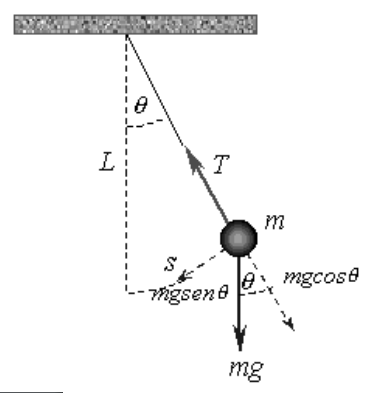
\includegraphics[width=7cm, height=6cm]{Pendulo.png}
  \caption{P\'endulo Simple}
\end{figure}

\newpage
Las fuerzas que act\'uan sobre la masa $m$ son la tensi\'on $T$ de la cuerda y el peso $mg$ de la masa, se muestran en la figura 1. La componente tangencial del peso, $mg \sin{\theta}$, siempre apunta hacia $\theta = 0$, en direcci\'on opuesta la desplazamiento. Esta es la fuerza de restituci\'on, entonces puede escribirse la ecuaci\'on
de movimiento en la direcci\'on tangencial de la forma: 

$$F_{t} = -mg\sin{\theta} \quad \rightarrow \quad m\frac{d^{2}s}{dt^{2}} = -mg\sin{\theta}$$

donde $s$ es el desplazamiento medido a lo largo del arco de trayectoria y el signo menos indica que $F_{t}$ act\'ua opuesta al movimiento. Como $s = L\theta$ y $L$ es
constante, la ecuaci\'on se transforma en: 

$$\frac{d^{2}\theta}{dt^{2}} = -\frac{g}{L}\sin{\theta}$$

Como el lado derecho es proporcional a $\sin{\theta}$, y no solo a $\theta$, se concluye que el movimiento no es arm\'onico simple. Esa es una ecuaci\'on diferencial dif\'icil de resolver, por lo que se supone que el p\'endulo se mueve en pequeños desplazamientos,
tal que $\theta$ es pequeño, en este caso se puede usar la aproximaci\'on
$\sin{theta} \approx \theta$ y la ecuaci\'on diferencial del movimiento se reduce a: 

$$ \frac{d^{2}\theta}{dt^{2}} = -\frac{g}{L}\theta $$

que tiene la misma forma que la ecuaci\'on que describe al movimiento arm\'onico
simple, por lo que solo en esas condiciones el movimiento del p\'endulo es
un movimiento arm\'onico simple. Su soluci\'on es entonces: 

$$ \theta = A\cos{(\omega t + \delta)} $$

donde A es la amplitud que corresponde al m\'aximo desplazamiento angular y
$\omega$ es la frecuencia angular, de valor:

$$ \omega = \sqrt[]{\frac{g}{L}} $$

El per\'iodo del movimiento es:

$$ T = \frac{2\pi}{\omega} = 2\pi \sqrt[]{\frac{L}{g}}$$

El periodo y la frecuencia de un p\'endulo simple dependen solo de la longitud
de la cuerda y la aceleraci\'on de gravedad, y son independiente de la masa $m$
del p\'endulo. Esto significa que todos los p\'endulos simples de igual longitud
en el mismo lugar, oscilar\'an con el mismo periodo. 

\section*{Programa}

En esta secci\'on se mostrar\'a un c\'odigo para Python con el que podremos calcular la posici\'on de la masa $m$ de un p\'endulo simple as\'i como su velocidad angular dada las condiciones iniciales, tambi\'en se ver\'a que para diferentes valores en los par\'ametros $a$ y $b$ se obtendr\'an diferentes movimientos armónicos (sobre-amortiguado, cr\'iticamiente amortiguado y sub-amortiguado).\\

El c\'odigo que se utiliz\'o fue el siguiente

\begin{verbatim}
import numpy as np
>>> def pend(y, t, b, c):
...     theta, omega = y
...     dydt = [omega, -b*omega - c*np.sin(theta)]
...     return dydt
...
#Tomamos los valores de las constantes como b=0.25 y c=5.0
>>> b = 0.25
>>> c = 5

#Condiciones iniciales
>>> y0 = [np.pi - 0.1, 0.0]

#Nuestra gama de tiempos es
>>> t = np.linspace(0, 25, 101)

#Odeint para generar la solución
>>> from scipy.integrate import odeint
>>> sol = odeint(pend, y0, t, args=(b, c))

#La solución es un vector de la forma (101, 2)
>>> import matplotlib.pyplot as plt
>>> plt.plot(t, sol[:, 0], 'b', label='theta(t)')
>>> plt.plot(t, sol[:, 1], 'g', label='omega(t)')
>>> plt.legend(loc='best')
>>> plt.xlabel('t')
>>> plt.grid()
>>> plt.show()

\end{verbatim}

En este primer ejemplo el coeficiente de amortiguamiento $b$ fue de 0.25, y nos imprimi\'o la gr\'afica caracter\'istica a un movimiento oscilatorio sub-amortiguado:

\vspace*{0.5cm}
\begin{figure}[!ht]
  \centering
      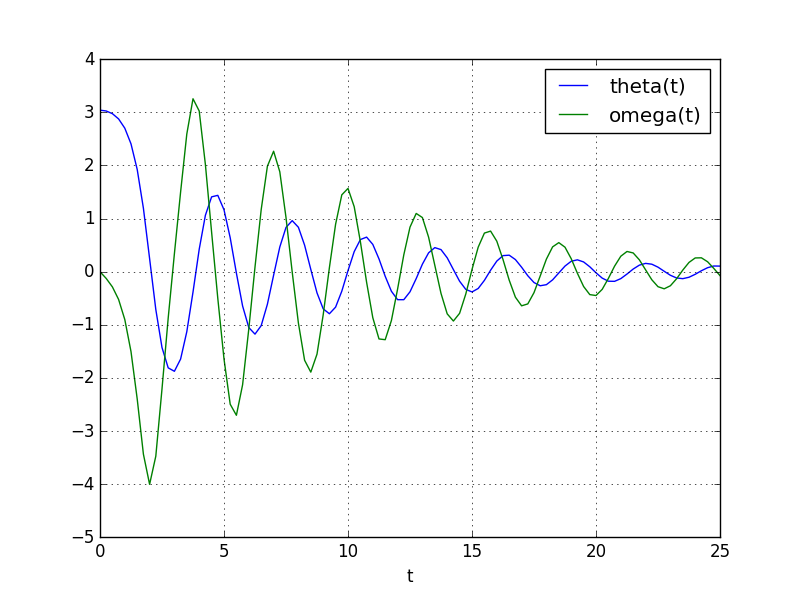
\includegraphics[width=7cm, height=6cm]{MovimientoAmortiguado.png}
  \caption{Movimiento Sub-amortiguado b=0.25 c=5}
\end{figure}

En la siguiente modificaci\'on se logr\'o que no hubiera fricci\'on en el movimiento (b=0), as\'i se obtuvo la siguiente gr\'afica:

\begin{figure}[!ht]
  \centering
      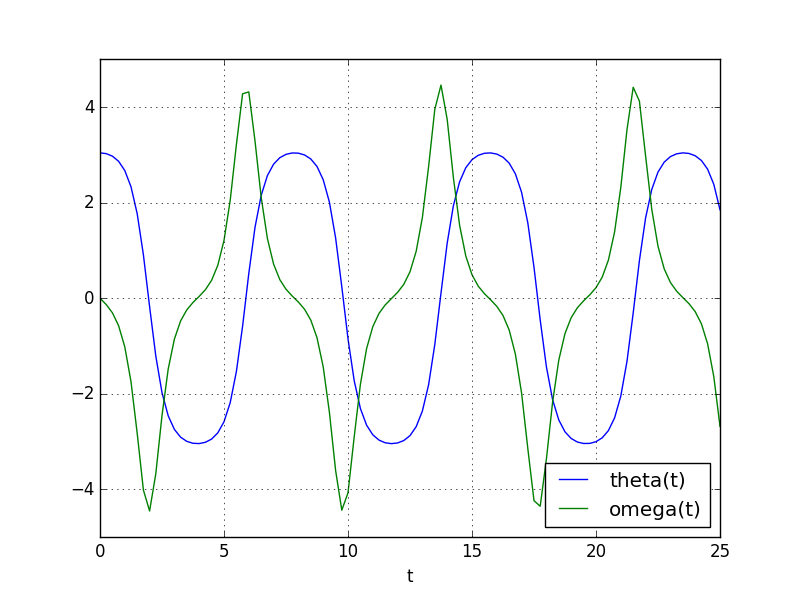
\includegraphics[width=7cm, height=6cm]{NoFriction.png}
  \caption{Movimiento sin fricci\'on b=0 c=5}
\end{figure}

\newpage

Claramente podemos observar que debido a que no hay fricci\'on la energ\'ia se conserva por ende el desplazamiento es el mismo en cada periodo transcurrido.\\

Ahora se modific\'o el c\'odigo para tener un movimiento cr\'iticamente-amortiguado (b=10 y c=5):

\begin{figure}[!ht]
  \centering
      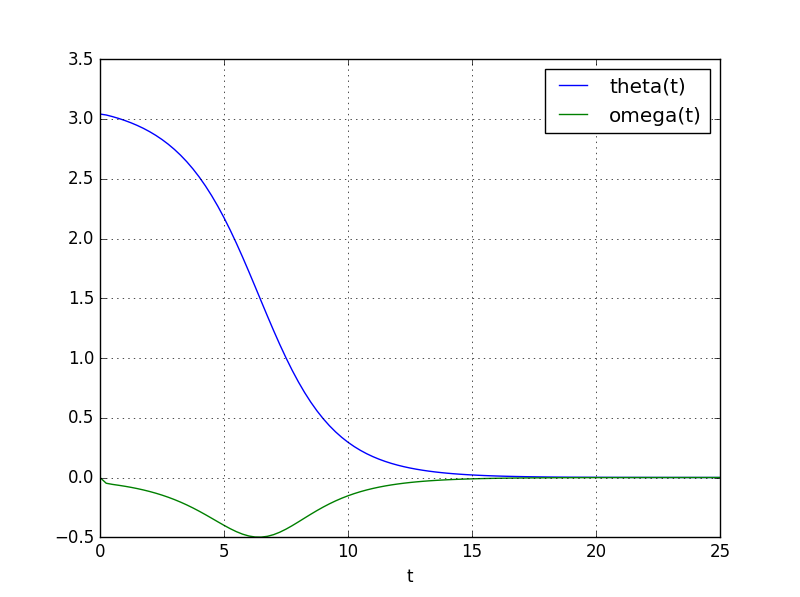
\includegraphics[width=7cm, height=6cm]{CriticamenteAmortiguado.png}
  \caption{Movimiento cr\'itico-amortiguado b=10 c=5}
\end{figure}

y por \'ultimo tenemos el movimiento sobre-amortiguado:


\begin{figure}[!ht]
  \centering
      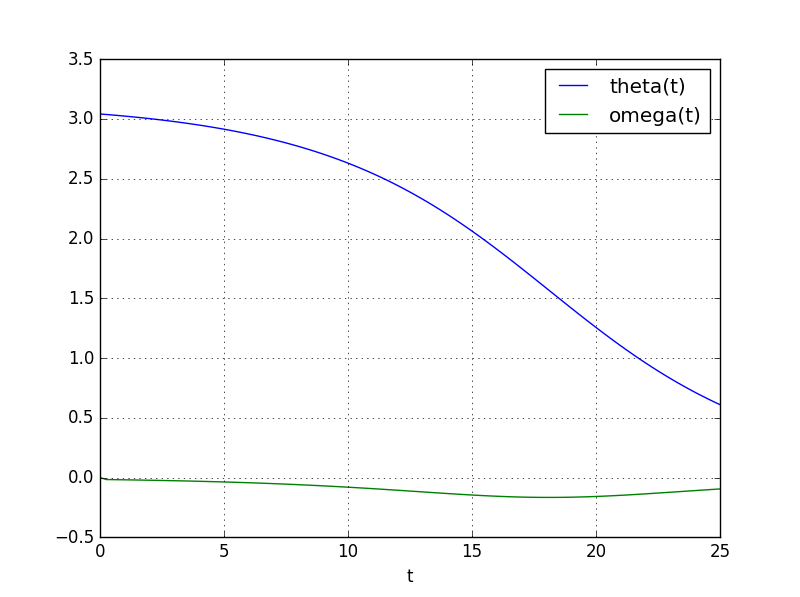
\includegraphics[width=7cm, height=6cm]{SobreAmortiguado.png}
  \caption{Movimiento Sobre-amortiguado b=30 c=5}
\end{figure}

\section*{Conclusi\'on}

En esta pr\'actica se aprendi\'o m\'as sobre el programa Python y logr\'o manipular un modelo f\'isico y jugar con sus par\'ametros para observar diferentes casos que se suelen presentar en la vida real.




\end{document}